\documentclass{OFbook}
\setcounter{secnumdepth}{4}
\nofiles

\usepackage[dvipdfm]{color}
\usepackage[dvipdfm]{graphicx}
\usepackage{mediabb}
\graphicspath{{./fig/pdf/}{./fig/png/}}
\usepackage{ltxtable}

\usepackage[deluxe]{otf}
\usepackage{lmodern}
\usepackage[T1]{fontenc}
\usepackage{textcomp}
\usepackage[utf8]{inputenc}
\usepackage{amsmath,amssymb}
\usepackage{bm}

\usepackage[dvipdfm,
 bookmarks=true,
 bookmarksnumbered=true,
 pdftitle={OpenFOAM Programmer's Guide},
 pdfsubject={Japanese edition},
 pdfauthor={The Open CAE Society of Japan (www.opencae.jp)},
 pdfkeywords={OpenFOAM},
 colorlinks=true,
 linkcolor=red,
 filecolor=blue,
 urlcolor=blue
 ]{hyperref}[2007/12/08]
\usepackage{atbegshi}
\AtBeginShipoutFirst{\special{pdf:tounicode EUC-UCS2}}

\usepackage{OFmacros}

\usepackage{makeidx}
\makeindex
\def\seename{$\Longrightarrow$}

\title{プログラマズガイド和訳}
\author{一般社団法人 オープンCAE学会}
\version{2.1.1}
\def\thepage{P-\arabic{page}}

\begin{document}

\maketitle
\frontmatter

\begin{OFdeclaration}
 %#! platex UserGuideJa


Copyright \copyright{} 2000, 2001, 2002, 2003, 2004, 2005, 2006, 2007, 2008, 2009 OpenCFD Limited.

\vskip\Cvs

Permission is granted to copy, distribute and/or modify this document under the terms
of the GNU Free Documentation License, Version 1.2 published by the Free Software
Foundation; with no Invariant Sections, no Back-Cover Texts and one Front-Cover Text:
``Available free from openfoam.org.'' A copy of the license is included in the section
entitled ``GNU Free Documentation License''.

\vskip\Cvs

This document is distributed in the hope that it will be useful, but WITHOUT ANY
WARRANTY; without even the implied warranty of MERCHANTABILITY or FITNESS
FOR A PARTICULAR PURPOSE.

\vskip2\Cvs

上記に示した英語版原文の著作権表示に従い,
GNU Free Documentation Licenseのバージョン1.2に基づいて,
本和訳文書の複製・配布・改変が許可されています.

\vskip.5\Cvs

次ページ以降にGNU Free Documentation Licenseを掲載します.

\vskip\Cvs

\hfill OpenFOAMユーザー会\par
\hfill 一般社団法人 オープンCAE学会\par

\vskip\Cvs

\noindent
Typeset in p\LaTeX.

 %#! uplatex UserGuideJa

\section*{Trademarks}
\OFthirdparty{ANSYS} is a registered trademark of ANSYS Inc.\par
\OFthirdparty{CFX} is a registered trademark of Ansys Inc.\par
\OFthirdparty{CHEMKIN} is a registered trademark of Reaction Design Corporation\par
\OFthirdparty{EnSight} is a registered trademark of Computational Engineering International Ltd.\par
\OFthirdparty{Fieldview} is a registered trademark of Intelligent Light\par
\OFthirdparty{Fluent} is a registered trademark of Ansys Inc.\par
\OFthirdparty{GAMBIT} is a registered trademark of Ansys Inc.\par
\OFthirdparty{Icem-CFD} is a registered trademark of Ansys Inc.\par
\OFthirdparty{I-DEAS} is a registered trademark of Structural Dynamics Research Corporation\par
\OFthirdparty{JAVA} is a registered trademark of Sun Microsystems Inc.\par
\OFthirdparty{Linux} is a registered trademark of Linus Torvalds\par
OpenFOAM is a registered trademark of ESI Group.\par
\OFthirdparty{ParaView} is a registered trademark of Kitware\par
\OFthirdparty{STAR-CD} is a registered trademark of Computational Dynamics Ltd.\par
\OFthirdparty{UNIX} is a registered trademark of The Open Group\par

\end{OFdeclaration}

\tableofcontents

\mainmatter
%#! platex ProgrammersGuideJa
\chapter{テンソル数学}
\label{chap:1}
この章では,
\index{テンソル}%
テンソルとそれらの代数演算について,
また本書におけるそれらの数学表記について記述します.
そして,テンソルおよびテンソル
\index{テンソル!すうがく@数学}%
数学がOpenFOAMにおいて
どのようにプログラムされているかを説明します.



\section{座標系}
\label{sec:1.1}
OpenFOAMは,主に
\index{れんぞくたい@連続体!りきがく@力学}%
連続体力学,
つまり固体・液体・気体の応力や,
これらの物質の変形や流れに関する力学分野の問題
を解くために設計されています.
このためOpenFOAMは,3次元空間と時間,
そして物理的要素のテンソルによる記述に基づいています.
OpenFOAMで使われる
\index{ざひょうけい@座標系}%
座標系は,
\autoref{fig:1.1}に示すような右手系デカルト座標系です.
この座標系は,$Ox$,$Oy$,$Oz$と名づけられた互いに直角な三つの軸から
原点$O$を定義することによって構成されます.
右手系とは,$O$から$Oz$軸のほうを見下ろしたとき,
$Ox$軸上の点から$Oy$軸上の点へと向かう円弧が
時計回りにみえるように定義されます.


\begin{figure}[ht]
 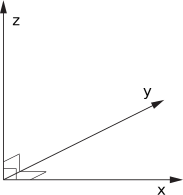
\includegraphics{fig-1-1}
 \caption{右手系座標軸}
 \label{fig:1.1}
\end{figure}



\section{テンソル}
\label{sec:1.2}
テンソル項は,特定の空間に属していて特定の数学的規則に従うような
実体について記述します.
簡潔にいえば,テンソルは単位基底ベクトルの組に対する
成分値の組で表現されます.
OpenFOAMではこの単位基底ベクトルは,
\index{ざひょうじく@座標軸!みぎてけいデカルトざひょうけい@右手系デカルト座標系}%
右手系デカルト座標軸$x$,$y$,$z$にそれぞれ沿った
$\mathbf{e}_{x}$,$\mathbf{e}_{y}$,$\mathbf{e}_{z}$になります.
したがって,これらの基底ベクトルは直交,すなわち互いに直角です.
すべてのテンソルは以下のような属性をもっています.
\begin{description}
 \item[次元] そのテンソルが属する特定の空間の次元$d$.
            OpenFOAMでは$d = 3$
 \item[ランク]
\index{テンソル!ランク}%
            成分値の数が$d^{r}$となるような整数$r \ge 0$
\end{description}
OpenFOAM~1.xが3
\index{テンソル!じげん@次元}%
次元であることから,
ランク$0$〜$3$のテンソルが標準で用意されていますが,
この基本のランクの設定は自由に拡張できるように書かれています.
ランク$0$と$1$のテンソルは,
\index{スカラ}%
スカラおよび
\index{ベクトル}%
ベクトルとしてのほうが
よく知られており読者にも身近でしょうが,
ランク$2$と$3$のテンソルにはあまりなじみがないかもしれません.
確認のために,OpenFOAM~1.xが標準で提供している
すべてのランクのテンソルを以下で復習しておきましょう.
\begin{description}
 \item[ランク0「スカラ」] 一つの実数で表せるあらゆる物理量で,
            イタリック体で表記されます.
            例えば,質量$m$,体積$V$,圧力$p$,そして粘性係数$\mu$です.
 \item[ランク1「ベクトル」] 大きさと方向で表現できる物理量です.
            成分表示では,ベクトル$\bm{a} = (a_{1},\ a_{2},\ a_{3})$は
            デカルト座標系の$x$軸,$y$軸,$z$軸成分をそれぞれ表します.
            同じベクトルを添字表記では$a_{i}$,$i = 1,\ 2,\ 3$と書けます.
            ただし,3次元を扱っていることは明らかなので
            本書では添字リスト$i = 1,\ 2,\ 3$は省略します.
 \item[ランク2「テンソル」] または
\index{テンソル!2かい@2階}%
「2階のテンソル」$\bm{T}$は
            以下のように行列で表現できる9\nobreak 個の要素をもっています.
            \begin{align}
             \label{eq:1.1}
             \bm{T} &= T_{ij}
             = \begin{pmatrix}
                T_{11} & T_{12} & T_{13} \\
                T_{21} & T_{22} & T_{23} \\
                T_{31} & T_{32} & T_{33}
               \end{pmatrix}
            \end{align}
            $r = 2$なので,要素$T_{ij}$は二つの添字で表されます.
            以下では添字のリスト$i,\ j = 1,\ 2,\ 3$は省略します.
            $i = j$の要素は対角要素とよばれ,
            $i \ne j$の要素は非対角要素とよばれます.
            対角要素を交差して要素を入れ替えることにより,
            以下のような$\bm{T}$の
\index{テンソル!てんち@転置}%
            \emph{転置}が得られます.
            \begin{align}
             \label{eq:1.2}
             \bm{T}^{\mathrm{T}} &= T_{ji}
             = \begin{pmatrix}
                T_{11} & T_{21} & T_{31} \\
                T_{12} & T_{22} & T_{32} \\
                T_{13} & T_{23} & T_{33}
               \end{pmatrix}
            \end{align}
            注意:ランク3以上のテンソルが出現することは非常にまれなので,
            多くの場合,ランク2のテンソルは単に「テンソル」とよばれます.
 \item[ランク2(対称)]
\index{テンソル!2かいたいしょう@2階対称}%
            「対称」というのは,対角方向に対称,
            つまり$T_{ij} = T_{ji}$であることを表します.
            この場合$T_{12} = T_{21}$,$T_{13} = T_{31}$,
            $T_{23} = T_{32}$なので,独立な要素は6個だけになります.
            対称テンソルであれば9個より6個の要素を保存するほうがメモリを節約できるので,
            OpenFOAMでは対称テンソルと非対称テンソルを区別して扱います.
            連続体力学において遭遇するほとんどのテンソルは対称です.
 \item[ランク3]
\index{テンソル!3かい@3階}%
            27個の要素をもち,添字表記では$P_{ijk}$と書けますが,
            \autoref{eq:1.1}\hskip\xkanjiskip のように行列表示しようとすると非常に長くなります.
\item[ランク3(対称)]
\index{テンソル!3かいたいしょう@3階対称}%
           ランク3の対称テンソルは,OpenFOAMでは
           $P_{ijk} = P_{ikj} = P_{jik} = P_{jki} = P_{kij} = P_{kji}$として定義されており,
           したがって10個の独立した要素をもちます.
           さらに厳密にいえば,これは相等しい三つのベクトルの外積によってつくられます.
           外積については\autoref{ssec:1.3.4}で述べられています.
\end{description}


\subsection{テンソル表記}
\label{ssec:1.2.1}
本書は,空間3次元と時間からなる複雑な偏微分方程式の問題を扱う,数値連続体力学に関するものです.
まず最初に,簡潔でありながら明確な,方程式の表記方法を導入しておくことが不可欠です.
方程式を追いやすいようにするには,スカラ要素のリストを書くよりも,
それ自体にテンソルの概念が含められた一つのもので表記することが必要です.
加えて,あらゆるテンソル演算が,要素それぞれに体する演算ではなく
テンソル自体に対する演算である,とわかるような表記法であるべきです.

そういうわけで,この文書ではランク1以上のテンソル,
すなわちスカラ以外のすべてのテンソルについては
\index{テンソル!ひょうき@表記}%
\emph{テンソル表記}を採用し,
太字で,例えば$\bm{a}$のように表記します.
これは一つのシンボルで表され,非常にコンパクトであることから,
それ自体で一つの存在としてテンソルを把握しやすくなります.
欠点をあげるとすれば,太字のシンボルはランク0でないことは明らかですが,
そのランクがすぐには読み取れないことです.
しかしながら,シンボルを見れば何の物理量を表しているかがわかり,
直観的にランクもわかるので,実際にはそれほど問題になりません.
例えば,私たちは速度$\bm{U}$がランク1のテンソルであることを知っています.

さらにいえば,表記方法の選択を評価するもっと根本的な点は,
テンソルの数学的表現が座標系によって変化しないこと,
つまりベクトル$\bm{a}$がどこから観測するかに拘らず
同じベクトルであることです.
テンソル表記は,座標系に関する情報をいっさい含まないので,
このコンセプトに合っています.
しかし,他の表記,たとえば$a_{i}$のようにテンソルの成分個別の表示は
必然的に座標系の選択を意味してしまいます.
この望ましくない結果は,
一意でない,つまり座標系に依存する
値の組み合わせでテンソルが表現されることによります.

とはいえ本書では,主にテンソル演算を成分要素に展開するために,
\autoref{sec:1.2}で述べたような添字表記もときどき用います.
添字表記を用いる際には,和の規約を採用します.
これは,一つの項に同じ添字が2回現れたら,
その添字については該当する全ての数字,たとえば$1$,$2$,$3$をとり,
それらの和をとるというものです.
たとえば次のようになります.
\begin{align}
 \label{eq:1.3}
 a_{i}b_{i} = \sum^{3}_{i=1}a_{i}b_{i} = a_{1}b_{1} + a_{2}b_{2} + a_{3}b_{3}
\end{align}

添字が繰り返されたら和を意味するので,この文書では今後,記号$\sum$は省略します.



\section{テンソルの代数演算}
\label{sec:1.3}
この節では,OpenFOAMで利用できるテンソルの
\index{テンソル!だいすうえんざん@代数演算}%
代数演算をすべて紹介します.
まず,もっとも基本的なテンソル演算をおさらいしておきましょう.
\index{テンソル!かさん@加算}%
加算,
\index{テンソル!げんさん@減算}%
減算,そして
\index{テンソル!スカラのじょうさん@スカラの乗算}%
スカラの乗算と除算です.
加算と減算は,可換則と結合則の両方を満たし,
互いにランクの等しいテンソルどうしに限って意味をもちます.
これはテンソルの要素それぞれについて加算・減算を行う操作であり,
たとえば,二つのベクトル$\bm{a}$と$\bm{b}$の差は
\begin{align}
 \label{eq:1.4}
 \bm{a} - \bm{b} = a_{i} - b_{i} = (a_{1} - b_{1},\ a_{2} - b_{2},\ a_{3} - b_{3})
\end{align}
となります.
テンソル$\bm{a}$にスカラ$s$をかける乗算も同様に可換則と結合則を満たし,
テンソルの要素すべてにスカラを乗じる操作です.
たとえば,次のようになります.
\begin{align}
 \label{eq:1.5}
 s\bm{a} = sa_{i} = (sa_{1},\ sa_{2},\ sa_{3})
\end{align}
テンソル$\bm{a}$と
\index{テンソル!スカラのじょさん@スカラの除算}%
スカラの除算は,
スカラが演算の第2引数となっているときにのみ意味をもちます.
つまり,次のとおりです.
\begin{align}
 \label{eq:1.6}
 \frac{\bm{a}}{s} = \frac{a_{i}}{s}
 = \left(\frac{a_{1}}{s},\ \frac{a_{2}}{s},\ \frac{a_{3}}{s}\right)
\end{align}
これ以降の節で述べる上記以外の演算は,
ランク1以上のテンソルどうしの,
さらに複雑な積の組み合わせとなっています.


\subsection{内積}
\label{ssec:1.3.1}
\index{テンソル!ないせき@内積}%
内積は,ランク$r_{1}$と$r_{2}$の任意の二つのテンソルを
ランク$r = r_{1} + r_{2} - 2$のテンソルにする演算です.
ランク3までのテンソルの内積演算を以下に示します.
\begin{itemize}
 \item 二つのベクトル$\bm{a}$と$\bm{b}$の内積は可換であり,
       以下のスカラ$s = \bm{a} \inProd \bm{b}$をつくります.
       \begin{align}
        \label{eq:1.7}
        s = a_{i}b_{i} = a_{1}b_{2} + a_{2}b_{2} + a_{3}b_{3}
       \end{align}
 \item テンソル$\bm{T}$とベクトル$\bm{a}$の内積は
       ベクトル$\bm{b} = \bm{T} \inProd \bm{a}$をつくります.
       これは,見やすいように列ベクトルで書くと,以下のようになります.
       \begin{align}
        \label{eq:1.8}
        b_{i} = T_{ij}a_{j} =
        \begin{pmatrix}
         T_{11}a_{1} + T_{12}a_{2} + T_{13}a_{3} \\
         T_{21}a_{1} + T_{22}a_{2} + T_{23}a_{3} \\
         T_{31}a_{1} + T_{32}a_{2} + T_{33}a_{3}
        \end{pmatrix}
       \end{align}
       もし$\bm{T}$が対称でなければ,
       $\bm{b} = \bm{a} \inProd \bm{T} = \bm{T}^{\mathrm{T}} \inProd \bm{a}$は
       以下のようになり,この演算は可換ではありません.
       \begin{align}
        \label{eq:1.9}
        b_{i} = a_{j}T_{ji} =
        \begin{pmatrix}
         a_{1}T_{11} + a_{2}T_{21} + a_{3}T_{31} \\
         a_{1}T_{12} + a_{2}T_{22} + a_{3}T_{32} \\
         a_{1}T_{13} + a_{2}T_{23} + a_{3}T_{33}
        \end{pmatrix}
       \end{align}
 \item 二つのテンソル$\bm{T}$と$\bm{S}$の内積は,
       以下のような成分をもつテンソル$\bm{P} = \bm{T} \inProd \bm{S}$をつくります.
       \begin{align}
        \label{eq:1.10}
        P_{ij} = T_{ik}S_{kj}
       \end{align}
       これは$\bm{T} \inProd \bm{S} =
       (\bm{S}^{\mathrm{T}} \inProd \bm{T}^{\mathrm{T}})^{\mathrm{T}}$となり,非可換です.
 \item ベクトル$\bm{a}$と3階のテンソル$\bm{P}$の内積は,
       以下のような成分をもつ2階のテンソル$\bm{T} = \bm{a} \inProd \bm{P}$をつくります.
       \begin{align}
        \label{eq:1.11}
        T_{ij} = a_{k}P_{kij}
       \end{align}
       やはりこれも非可換で,
       $\bm{T} = \bm{P} \inProd \bm{a}$は次のようになります.
       \begin{align}
        \label{eq:1.12}
        T_{ij} = P_{ijk}a_{k}
       \end{align}
 \item 2階のテンソル$\bm{T}$と3階のテンソル$\bm{P}$の内積は,
       以下のような成分をもつ3階のテンソル$\bm{Q} = \bm{T} \inProd \bm{P}$をつくります.
       \begin{align}
        \label{eq:1.13}
        Q_{ijk} = T_{il}P_{ljk}
       \end{align}
       やはりこれも非可換で,
       $\bm{Q} = \bm{P} \inProd \bm{T}$は次のようになります.
       \begin{align}
        \label{eq:1.14}
        Q_{ijk} = P_{ijl}T_{lk}
       \end{align}
\end{itemize}


\subsection{二つのテンソルの二重内積}
\label{ssec:1.3.2}
二つの2階テンソル$\bm{T}$と$\bm{S}$の
\index{テンソル!にじゅうないせき@二重内積}%
二重内積は,
スカラ$s = \bm{T} \biInProd \bm{S}$をつくります.
これは,テンソル成分の9個の積の和として得られます.
\begin{align}
 \label{eq:1.15}
 \begin{aligned}
  s = T_{ij}S_{ij} &= T_{11}S_{11} + T_{12}S_{12} + T_{13}S_{13} + {} \\
  &\hphantom{{}={}} T_{21}S_{21} + T_{22}S_{22} + T_{23}S_{23} + {} \\
  &\hphantom{{}={}} T_{31}S_{31} + T_{32}S_{32} + T_{33}S_{33}
 \end{aligned}
\end{align}

2階のテンソル$\bm{T}$と3階のテンソル$\bm{P}$の二重内積は,
次のような成分をもつベクトル$\bm{a} = \bm{T} \biInProd \bm{P}$をつくります.
\begin{align}
 \label{eq:1.16}
 a_{i} = T_{jk}P_{jki}
\end{align}
これは非可換で,$\bm{a} = \bm{P} \biInProd \bm{T}$は次のようになります.
\begin{align}
 \label{eq:1.17}
 a_{i} = P_{ijk}T_{jk}
\end{align}


\subsection{二つの3階テンソルの三重内積}
\label{ssec:1.3.3}
二つの3階テンソル$\bm{P}$と$\bm{Q}$の
\index{テンソル!さんじゅうないせき@三重内積}%
三重内積は,
スカラ$s = \bm{P} \triInProd \bm{Q}$をつくります.
これは,テンソル成分の27個の積の和として得られます.
\begin{align}
 \label{eq:1.18}
 \begin{aligned}
  s = P_{ijk}Q_{ijk}
 \end{aligned}
\end{align}


\subsection{外積}
\label{ssec:1.3.4}
\index{テンソル!がいせき@外積}%
外積は,以下のようなベクトルやテンソルどうしの演算です.
\begin{itemize}
 \item 二つのベクトル$\bm{a}$と$\bm{b}$の外積は非可換で,
       以下のような成分をもつテンソル
       $\bm{T} = \bm{a}\bm{b} = (\bm{b}\bm{a})^{\mathrm{T}}$をつくります.
       \begin{align}
        \label{eq:1.19}
        T_{ij} = a_{i}b_{j} =
        \begin{pmatrix}
         a_{1}b_{1} & a_{1}b_{2} & a_{1}b_{3} \\
         a_{2}b_{1} & a_{2}b_{2} & a_{2}b_{3} \\
         a_{3}b_{1} & a_{3}b_{2} & a_{3}b_{3}
        \end{pmatrix}
       \end{align}
 \item ベクトル$\bm{a}$と2階のテンソル$\bm{T}$との外積は,
       以下のような成分をもつ3階のテンソル
       $\bm{P} = \bm{a}\bm{T}$をつくります.
       \begin{align}
        \label{eq:1.20}
        P_{ijk} = a_{i}T_{jk}
       \end{align}
       これは非可換で,
       $\bm{P} = \bm{T}\bm{a}$は以下のようになります.
       \begin{align}
        \label{eq:1.21}
        P_{ijk} = T_{ij}a_{k}
       \end{align}
\end{itemize}


\subsection{二つのベクトルのクロス積}
\label{ssec:1.3.5}
\index{テンソル!ベクトルのクロスせき@ベクトルのクロス積}%
クロス積はベクトルだけに存在する演算です.
二つのベクトル$\bm{a}$と$\bm{b}$について,
これらのクロス積は以下のような成分をもつベクトル
$\bm{c} = \bm{a} \times \bm{b}$をつくります.
\begin{align}
 \label{eq:1.22}
 c_{i} = e_{ijk}a_{j}b_{k}
 = (a_{2}b_{3} - a_{3}b_{2},\ a_{3}b_{1} - a_{1}b_{3},\  a_{1}b_{2} - a_{2}b_{1})
\end{align}
ここで
\index{ちかんきごう@置換記号}%
\OFemph{置換記号}は以下のように定義されます.
\begin{align}
 \label{eq:1.23}
 e_{ijk} =
 \begin{cases}
  0 & \text{いずれか二つの添字が等しいとき} \\
  +1 & \text{$i,\ j,\ k$が$1,\ 2,\ 3$の偶置換のとき} \\
  -1 & \text{$i,\ j,\ k$が$1,\ 2,\ 3$の奇置換のとき}
 \end{cases}
\end{align}
偶置換とは$123$,$231$および$312$であり,
奇置換は$132$,$213$および$321$です.


\subsection{その他の一般的なテンソル演算}
\label{ssec:1.3.6}
OpenFOAMで使われる,やや一般的でない演算や専門用語を以下に示します.
\begin{description}
 \item[二乗]
\index{テンソル!にじょう@二乗}%
            テンソルの二乗は,それ自身とのテンソル外積で定義されます.
            例えば,ベクトル$\bm{a}$の二乗は$\bm{a}^{2} = \bm{a}\bm{a}$です.
 \item[$n$乗]
\index{テンソル!nじょう@$n$乗}%
            テンソルの$n$乗は,それ自身との$n$回のテンソル外積で定義されます.
            例えば,ベクトル$\bm{a}$の$3$乗は$\bm{a}^{3} = \bm{a}\bm{a}\bm{a}$です.
 \item[平方絶対値]
\index{テンソル!へいほうぜったいち@平方絶対値}%
            テンソルの平方絶対値は,それ自身との$r$テンソルの$r$重内積で,スカラとなります.
            例えば,2階テンソル$\bm{T}$については,$|\bm{T}|^{2} = \bm{T} \biInProd \bm{T}$です.
 \item[絶対値]
\index{テンソル!ぜったいち@絶対値}%
            平方絶対値の平方根です.
            例えば,テンソル$\bm{T}$については,$|\bm{T}| = \sqrt{\bm{T} \biInProd \bm{T}}$です.
            単位長さのベクトルは
\index{ベクトル!たんい@単位}%
            \OFemph{単位ベクトル}とよばれます.
 \item[最大成分]
\index{テンソル!さいだいせいぶん@最大成分}%
            符号も考慮した最大の値をもつテンソルの成分です.つまり最大の絶対値ではありません.
 \item[最小成分]
\index{テンソル!さいしょうせいぶん@最小成分}%
            最小の値をもつテンソルの成分です.
 \item[成分平均値]
\index{テンソル!せいぶんへいきんち@成分平均値}%
            テンソルのすべての成分の平均値です.
 \item[スケール] 名前のとおり,
\index{テンソル!スケールかんすう@スケール関数}%
            スケール関数は,
            あるテンソルの成分を同じランクの他のテンソルの成分でスケーリングします.
            これは二つのテンソルの対応する成分同士の積で評価されます.
            例えば,ベクトル$\bm{a}$のベクトル$\bm{b}$によるスケーリングは,
            以下のような成分のベクトル$\bm{c}$をつくります.
            \begin{align}
             \label{eq:1.24}
             c_{i} = \mathop{\mathrm{scale}}(\bm{a},\ \bm{b})
             = (a_{1}b_{1},\ a_{2}b_{2},\ a_{3}b_{3})
            \end{align}
\end{description}


\subsection{幾何変換と単位テンソル}
\label{ssec:1.3.7}
2階のテンソル$\bm{T}$は線形ベクトル関数,
すなわち,内積$\bm{b} = \bm{T} \inProd \bm{a}$によって,
あるベクトル$\bm{a}$を別のベクトル$\bm{b}$に結びつける関数として,
厳密に定義されます.
$x,\ y,\ z$座標系から新しい座標系$x^{*},\ y^{*},\ z^{*}$への
あるテンソルの座標
\index{テンソル!きかへんかん@幾何変換}%
\index{テンソル!へんかん@変換}%
変換として機能するように,
$\bm{T}$の成分を選ぶことができます.
このとき$\bm{T}$を\OFemph{変換テンソル}とよびます.
スカラは変換によって変化しませんが,
ベクトル$\bm{a}$は
\begin{align}
 \label{eq:1.25}
 \bm{a}^{*} = \bm{T} \inProd \bm{a}
\end{align}
のように$\bm{a}^{*}$に変換されます.
2階のテンソル$\bm{S}$は
\begin{align}
 \label{eq:1.26}
 \bm{S}^{*} = \bm{T} \inProd \bm{S} \inProd \bm{T}^{\mathrm{T}}
\end{align}
に従って$\bm{T}^{*}$に変換されます.

\index{テンソル!たんい@単位}%
\OFemph{単位テンソル}$\bm{I}$は,
あるテンソルをそれ自身に変換するという条件から定義されます.
すべてのベクトル$\bm{a}$に対して
\begin{align}
 \label{eq:1.27}
 \bm{a} = \bm{I} \inProd \bm{a}
\end{align}
となり,つまり
\begin{align}
 \label{eq:1.28}
 \bm{I} = \delta_{ij} =
 \begin{pmatrix}
  1 & 0 & 0 \\
  0 & 1 & 0 \\
  0 & 0 & 1 \\
 \end{pmatrix}
\end{align}
となります.ここで,$\delta_{ij}$は
\index{クロネッカーのデルタ}%
\OFemph{クロネッカーのデルタ}として知られています.


\subsection{便利なテンソルの恒等式}
\label{ssec:1.3.8}
さまざまな
\index{テンソル!こうとうしき@恒等式}%
恒等式を以下に示します.
これらは,関連するすべての微分が存在して連続であるという仮定のもとで証明できます.
スカラ$s$とベクトル$\bm{a}$および$\bm{b}$を用いて表記しています.
%%% 訳注:原文では$\bm{b}$への言及が抜けている.
\begin{align}
 \label{eq:1.29}
 \begin{aligned}
  \nabla \inProd (\nabla \times \bm{a}) &\equiv 0 \\
  \nabla \times (\nabla s) &\equiv \bm{0} \\
  \nabla \inProd (s\bm{a}) &\equiv s\nabla \inProd \bm{a} + \bm{a} \inProd \nabla s \\
  \nabla \times (s\bm{a}) &\equiv s\nabla \times \bm{a} + \nabla s \times \bm{a} \\
  \nabla (\bm{a} \inProd \bm{b})
    &\equiv \bm{a} \times (\nabla \times \bm{b}) + \bm{b} \times (\nabla \times \bm{a})
            + (\bm{a} \inProd \nabla)\bm{b} + (\bm{b} \inProd \nabla)\bm{a} \\
  \nabla \inProd (\bm{a} \times \bm{b})
    &\equiv \bm{b} \inProd (\nabla \times \bm{a}) - \bm{a} \inProd (\nabla \times \bm{b}) \\
  \nabla \times (\bm{a} \times \bm{b})
    &\equiv \bm{a}(\nabla \inProd \bm{b}) - \bm{b}(\nabla \inProd \bm{a})
            + (\bm{b} \inProd \nabla)\bm{a} - (\bm{a} \inProd \nabla)\bm{b} \\
  \nabla \times (\nabla \times \bm{a})
    &\equiv \nabla (\nabla \inProd \bm{a}) - \Laplacian\bm{a} \\
  (\nabla \times \bm{a})
    &\equiv \bm{a} \inProd (\nabla \bm{a}) - \nabla (\bm{a} \inProd \bm{a})
 \end{aligned}
\end{align}
添字表記の数式を操作するときには,
以下の$e$--$\delta$恒等式を知っていると役立つことがあります.
\begin{align}
 \label{eq:1.30}
 e_{ijk}e_{irs} = \delta_{jr}\delta_{ks} - \delta_{js}\delta_{kr}
\end{align}


\subsection{2階テンソル特有の演算}
\label{ssec:1.3.9}
以下に示すように,2階テンソルの成分を操作する様々な演算があります.
\begin{description}
 \item[転置]
\index{テンソル!てんち@転置}%
            \autoref{eq:1.2}で示したように,
            テンソル$\bm{T} = T_{ij}$の転置は$\bm{T}^{\mathrm{T}} = T_{ji}$です.
 \item[対称テンソルと歪(反対称)テンソル] \autoref{sec:1.2}で述べたように,
            $\bm{T} = \bm{T}^{\mathrm{T}}$のように
            成分が対角方向に対称なテンソルを
\index{テンソル!たいしょうテンソル@対称テンソル}%
            対称テンソルとよびます.
\index{テンソル!わいテンソル@歪テンソル}%
            歪テンソルもしくは
\index{テンソル!はんたいしょうテンソル@反対称テンソル|see{歪テンソル}}%
            反対称テンソルは$\bm{T} = -\bm{T}^{\mathrm{T}}$であり,
            当然$T_{11} = T_{22} = T_{33} = 0$となります.
            あらゆる2階テンソルは,以下のように対称テンソルと歪テンソルに分割できます.
            \begin{align}
             \label{eq:1.31}
             \bm{T} = \underbrace{\frac{1}{2}(\bm{T} + \bm{T}^{\mathrm{T}})}_{\text{対称テンソル}}
             + \underbrace{\frac{1}{2}(\bm{T} - \bm{T}^{\mathrm{T}})}_{\text{歪テンソル}}
             = \mathop{\mathrm{symm}}\bm{T} + \mathop{\mathrm{skew}}\bm{T}
            \end{align}
 \item[トレース] テンソル$\bm{T}$の
\index{テンソル!トレース}%
            トレースは対角成分の総和をとったスカラです.
            \begin{align}
             \label{eq:1.32}
             \mathop{\mathrm{tr}}\bm{T} = T_{11} + T_{22} + T_{33}
            \end{align}
 \item[対角] 2階テンソル$\bm{T}$の
\index{テンソル!たいかく@対角}%
            対角成分を成分とするベクトルを返します.
            \begin{align}
             \label{eq:1.33}
             \mathop{\mathrm{diag}}\bm{T} = (T_{11},\ T_{22},\ T_{33})
            \end{align}
 \item[偏差テンソルと静水圧テンソル] あらゆる2階テンソル$\bm{T}$は,
            $\mathop{\mathrm{tr}}T = 0$となる偏差成分と,
            スカラ$s$に対して$\bm{T} = s\bm{I}$となる静水圧成分に分割できます.
            あらゆる2階テンソルは,以下のように
\index{テンソル!へんさテンソル@偏差テンソル}%
            偏差テンソルと
\index{テンソル!せいすいあつテンソル@静水圧テンソル}%
            静水圧テンソルに分割できます.
            \begin{align}
             \label{eq:1.34}
             \bm{T} = \underbrace{\bm{T}
             - \frac{1}{3}(\mathop{\mathrm{tr}}\bm{T})\bm{I}}_{\text{偏差テンソル}}
             + \underbrace{\frac{1}{3}(\mathop{\mathrm{tr}}\bm{T})\bm{I}}_{\text{静水圧テンソル}}
             = \mathop{\mathrm{dev}}\bm{T} + \mathop{\mathrm{hyd}}\bm{T}
            \end{align}
 \item[行列式] 2階テンソルの
\index{テンソル!ぎょうれつしき@行列式}%
            行列式は以下で与えられます.
            \begin{align}
             \label{eq:1.35}
             \begin{split}
              \det\bm{T} &= \begin{vmatrix}
                             T_{11} & T_{12} & T_{13} \\
                             T_{21} & T_{22} & T_{23} \\
                             T_{31} & T_{32} & T_{33}
                            \end{vmatrix} \\
              &= T_{11}(T_{22}T_{33} - T_{23}T_{32})
              - T_{12}(T_{21}T_{33} - T_{23}T_{31})
              + T_{13}(T_{21}T_{32} - T_{22}T_{31}) \\
              &= \frac{1}{6}e_{ijk}e_{pqr}T_{ip}T_{jq}T_{kr}
             \end{split}
            \end{align}
 \item[余因子] テンソルのある成分が属する行と列を取り除いてできた部分を
            $2 \times 2$の行列式として評価したものを,
            テンソルのそれぞれの成分に対する小行列式といいます.
            例えば,$T_{12}$に対する小行列式は
            \begin{align}
             \label{eq:1.36}
             \begin{vmatrix}
              \rlap{\rule[4pt]{67pt}{.4pt}}T_{11} &
              \rlap{\hskip5pt\smash{\rule[-36pt]{.4pt}{44pt}}}T_{12} & T_{13} \\
              T_{21} & T_{22} & T_{23} \\
              T_{31} & T_{32} & T_{33}
             \end{vmatrix}
             = \begin{vmatrix}
                T_{21} & T_{23} \\
                T_{31} & T_{33}
               \end{vmatrix}
             = T_{21}T_{33} - T_{23}T_{31}
            \end{align}
            となります.
\index{テンソル!よいんし@余因子}%
            余因子とは,それぞれの成分の位置に応じて以下のルールで符号付けした小行列式です.
            \begin{align}
             \label{eq:1.37}
             \begin{aligned}
              &\text{$i + j$が偶数ならば$+$} \\
              &\text{$i + j$が奇数ならば$-$}
             \end{aligned}
            \end{align}
            $\bm{T}$の余因子は以下のようになります.
            \begin{align}
             \label{eq:1.38}
             \mathop{\mathrm{cof}}\bm{T} = \frac{1}{2}e_{jkr}e_{ist}T_{sk}T_{tr}
            \end{align}
 \item[逆元]
\index{テンソル!ぎゃくげん@逆元}%
            テンソルの逆元は以下で評価されます.
            \begin{align}
             \label{eq:1.39}
             \mathop{\mathrm{inv}}\bm{T}
             = \frac{\mathop{\mathrm{cof}}\bm{T}^{\mathrm{T}}}{\det\bm{T}}
            \end{align}
 \item[ホッジ双対]
\index{テンソル!ホッジそうつい@ホッジ双対}%
            テンソルのホッジ双対とは,以下のような成分をもつベクトルです.
            \begin{align}
             \label{eq:1.40}
             \mathop{*}\bm{T} = (T_{23},\ -T_{13},\ T_{12})
            \end{align}
\end{description}


\subsection{スカラ特有の演算}
\label{ssec:1.3.10}
OpenFOAMは,スカラを扱うよく知られた関数のほとんどをサポートしています.
例えば平方根,指数,対数,正弦,余弦などで,
これらのリストが\autoref{tbl:1.2}にあります.
OpenFOAMでは,これらに加えて以下の$3$種類の関数も定義されています.
\begin{description}
 \item[符号] スカラ$s$の符号は以下のように得られます.
            \begin{align}
             \label{eq:1.41}
             \mathop{\mathrm{sgn}}(s) =
             \begin{cases}
              1 & \text{$s \ge 0$のとき} \\
              -1 & \text{$s < 0$のとき}
             \end{cases}
            \end{align}
 \item[正数] スカラ$s$に対して以下のように得られます.
            \begin{align}
             \label{eq:1.42}
             \mathop{\mathrm{pos}}(s) =
             \begin{cases}
              1 & \text{$s \ge 0$のとき} \\
              0 & \text{$s < 0$のとき}
             \end{cases}
            \end{align}
 \item[制限] スカラ$s$のスカラ$n$による制限は以下のようになります.
            \begin{align}
             \label{eq:1.43}
             \mathop{\mathrm{limit}}(s,\ n) =
             \begin{cases}
              s & \text{$s < n$のとき} \\
              0 & \text{$s \ge n$のとき}
             \end{cases}
            \end{align}
\end{description}



\section{OpenFOAMのテンソルクラス}
\label{sec:1.4}
OpenFOAMには,これまでに述べたようなテンソル数学のためのクラス群を含んだ
\index{primitive@\OFclass{primitive}!ライブラリ}%
\index{ライブラリ!primitive@\OFclass{primitive}}%
\OFclass{primitive}というC++のクラスライブラリがあります.
OpenFOAMで標準的に使える基本テンソル
\index{テンソル!OpenFOAMにおけるクラス}%
クラスを\autoref{tbl:1.1}に列挙します.
この表にはテンソルの個別の成分にアクセスするための関数,
いわゆる
\index{アクセスかんすう@アクセス関数}%
アクセス関数も列挙してあります.


\begin{table}[ht]
 %#! uplatex ProgrammersGuideJa
\begin{tabular}{clll}
 ランク & 名称 & 基本クラス & アクセス関数 \\
 \hline
 \tblstrut
 $0$ & スカラ &
\index{クラス!scalar@\OFclass{scalar}}%
\index{scalarクラス@\OFclass{scalar}クラス}%
         \OFclass{scalar} & \\
 $1$ & ベクトル &
\index{クラス!vector@\OFclass{vector}}%
\index{vectorクラス@\OFclass{vector}クラス}%
         \OFclass{vector} & \OFkeyword{x()}, \OFkeyword{y()}, \OFkeyword{z()} \\
 $2$ & テンソル &
\index{クラス!tensor@\OFclass{tensor}}%
\index{tensorクラス@\OFclass{tensor}クラス}%
         \OFclass{tensor} & \OFkeyword{xx()}, \OFkeyword{xy()}, \OFkeyword{xz()}, ... \\
 \hline
\end{tabular}

 \caption{OpenFOAMにおける基本テンソルクラス}
 \label{tbl:1.1}
\end{table}


テンソル
\begin{align}
 \label{eq:1.44}
 \bm{T} =
 \begin{pmatrix}
  1 & 2 & 3 \\
  4 & 5 & 6 \\
  7 & 8 & 9
 \end{pmatrix}
\end{align}
は,OpenFOAMでは次の1行で宣言できます.
\begin{OFverbatim}[terminal]
tensor T(1, 2, 3, 4, 5, 6, 7, 8, 9);
\end{OFverbatim}

アクセス関数\OFkeyword{xz()}で
成分$T_{13}$つまり$T_{xz}$にアクセスできます.
例えば,コード
\begin{OFverbatim}[terminal]
Info << ``Txz = '' << T.xz() << endl;
\end{OFverbatim}
は,以下を画面に出力します.
\begin{OFverbatim}[terminal]
Txz = 3
\end{OFverbatim}


\subsection{OpenFOAMにおけるテンソルの代数演算}
\label{ssec:1.4.1}
\autoref{sec:1.3}で述べたすべての
\index{テンソル!OpenFOAMにおけるテンソルのだいすうえんざん@OpenFOAMにおけるテンソルの代数演算}%
代数演算は,
OpenFOAMのテンソルクラスに対して,
数学の表記法によく似た構文で利用できます.
いくつかの関数は,例えば\OFkeyword{symm()}のように,単に記述的な関数で表現しますが,
その他については,例えば\hskip\xkanjiskip\OFkeyword{*}\hskip\xkanjiskip のような演算子記号でも使用できます.
すべての関数を\autoref{tbl:1.2}に列挙します.


\vskip\floatsep
\begingroup
 \small
% \begin{table}[ht]
 \LTXtable{.8\textwidth}{tbl/tbl-1-2}
% 原文では,逆三角関数がプログラミング言語のように
% asin,acos,atan などとされているが,
% あまり数学で使われる表記ではないと思われるため,
% ここでは arcsin,arccos,arctan などとした.
 \addtocounter{table}{-1}%
 \tblcaption{OpenFOAMにおけるテンソルの代数演算}
 \label{tbl:1.2}
% \end{table}
\endgroup
\vskip\floatsep



\section{物理次元の単位}
\label{sec:1.5}
連続体力学では,物理量はある選ばれた単位で記述されます.
例えば,質量はキログラム ($\unit*{kg}$),
体積は立方メートル ($\unit*{m^{3}}$),
圧力はパスカル ($\unit*{kg\,m^{-1}\,s^{-2}}$).
これらの物理量に対する代数演算は,
\index{たんい@単位!けいりょう@計量}%
計量単位を一致させて行わなければなりません.
特に,加算,減算,等価判定は,同じ単位の物理量に対してのみ,物理的な意味をもちます.
無意味な演算の実装を予防するために,
\index{じげん@次元!OpenFOAMにおけるじげんチェック@OpenFOAMにおける次元チェック}%
OpenFOAMはユーザがあらゆるテンソルに物理次元の単位を付加することを推奨し,
これによりあらゆるテンソル演算の際に次元のチェックが行われます.

単位は,例えば以下のように,\OFclass{dimensionSet}クラスで定義されます.
\begin{OFverbatim}[terminal]
dimensionSet pressureDims(1, -1, -2, 0, 0, 0, 0);
\end{OFverbatim}


\begin{table}[ht]
 %#! platex ProgrammersGuideJa
\begin{tabular}{clll}
 No. & 物理量 & 単位 & 記号 \\
 \hline
 \tblstrut
 1 & 質量 & キログラム & $\mathrm{kg}$ \\
 2 & 長さ & メートル & $\mathrm{m}$ \\
 3 & 時間 & 秒 & $\mathrm{s}$ \\
 4 & 熱力学温度 & ケルビン & $\mathrm{K}$ \\
 5 & 物質量 & モル & $\mathrm{mol}$ \\
 6 & 電流 & アンペア & $\mathrm{A}$ \\
 7 & 光度 & カンデラ & $\mathrm{cd}$ \\
 \hline
\end{tabular}

 \caption{SI基本計量単位}
 \label{tbl:1.3}
\end{table}


ここで,それぞれの値は,\autoref{tbl:1.3}に列挙した
SI基本計量単位それぞれの指数を示しています.
このコードでは\OFkeyword{pressureDims}を,
圧力$\unit*{kg\,m^{-1}\,s^{-2}}$の\OFclass{dimensionSet}として宣言しています.
すなわち\OFkeyword{pressureDims}の引数配列の最初の項目$1$は$\unit*{kg^{1}}$を表し,
二つめの$-1$は$\unit*{m^{-1}}$を表す,などのようにです.
単位付きのテンソルは
\index{dimensioned<Type>@\OFclass{dimensioned<Type>}!テンプレートクラス}%
\OFclass{dimensioned<Type>}テンプレートクラスで定義されます.
\OFclass{<Type>}は\OFclass{scalar},\OFclass{vector},\OFclass{tensor}などです.
この
\index{テンプレートクラス!dimensioned<Type>@\OFclass{dimensioned<Type>}}%
\OFclass{dimensioned<Type>}は,
\index{word@\OFclass{word}!クラス}%
\index{クラス!word@\OFclass{word}}%
\OFclass{word}クラスの変数名,
\OFclass{<Type>}の値,そして
\index{クラス!dimensionSet@\OFclass{dimensionSet}}%
\index{dimensionSet@\OFclass{dimensionSet}!クラス}%
\OFclass{dimensionSet}を保持します.

\begin{OFverbatim}[terminal]
dimensionedTensor sigma
    (
        "sigma",
        dimensionSet(1, -1, -2, 0, 0, 0, 0),
        tensor(1e6, 0, 0, 0, 1e6, 0, 0, 0, 1e6),
    );
\end{OFverbatim}
は,圧力あるいは応力としてしかるべき次元をもつ以下のテンソルをつくります.
\begin{align}
 \label{eq:1.45}
 \sigma =
 \begin{pmatrix}
  10^{6} & 0 & 0 \\
  0 & 10^{6} & 0 \\
  0 & 0 & 10^{6} \\
 \end{pmatrix}
\end{align}


%#! platex ProgrammersGuideJa
\chapter{離散化手法}
\label{chap:2}
これまではテンソル代数について議論してきました.
我々が解きたい偏微分方程式は,テンソルの時間および空間に対する微分に関するものです.
したがって,\OFemph{テンソル場},すなわち時間および空間の領域にわたって変化するテンソルへと,
表現を拡張する必要があります.
この章では,まずはじめに登場するすべての微分演算の数学的表現を解説します.
そして,OpenFOAMではテンソル場がどのように構築されているのか,
これらの場の微分はどのようにして代数式へと離散化されるのかを紹介します.



\section{微分演算子}
\label{sec:2.1}
空間微分を定義する前に,ベクトル演算子ナブラ$\nabla$を紹介します.
添字表記では$\partial_{i}$と書かれます.
\begin{align}
 \label{eq:2.1}
 \nabla \equiv \partial_{i} \equiv \frac{\partial}{\partial x_{i}}
 \equiv \left(\frac{\partial}{\partial x_{1}},\
 \frac{\partial}{\partial x_{2}},\
 \frac{\partial}{\partial x_{3}}\right)
\end{align}
ナブラ演算子は,以下のルールに従う便利な表記法です.
\begin{itemize}
 \item テンソルに作用するときは,自身の右側に向かって,通常の積の微分のルールに従う.
       例えば$\partial_{i}ab = (\partial_{i}a)b + a(\partial_{i}b)$
 \item それ以外の場合,ナブラ演算子は代数演算における通常のベクトルと同様に振る舞う.
\end{itemize}


\subsection{勾配}
\label{ssec:2.1.1}
スカラ場$s$が定義されていて,連続微分可能ならば,
$s$の勾配$\nabla s$は以下のベクトル場となります.
\begin{align}
 \label{eq:2.2}
 \nabla s = \partial_{i}s
 = \left(\frac{\partial s}{\partial x_{1}},\
 \frac{\partial s}{\partial x_{2}},\
 \frac{\partial s}{\partial x_{3}}\right)
\end{align}

勾配はあらゆるテンソル場に作用し,一つランクの高いテンソル場を作ります.
例えば,ベクトル場$\bm{a}$の勾配は,以下の2階テンソルです.
\begin{align}
 \label{eq:2.3}
 \nabla\bm{a} = \partial_{i}a_{j} =
 \begin{pmatrix}
  \partial a_{1}/\partial x_{1} & \partial a_{2}/\partial x_{1} & \partial a_{3}/\partial x_{1} \\
  \partial a_{1}/\partial x_{2} & \partial a_{2}/\partial x_{2} & \partial a_{3}/\partial x_{2} \\
  \partial a_{1}/\partial x_{3} & \partial a_{2}/\partial x_{3} & \partial a_{3}/\partial x_{3} \\
 \end{pmatrix}
\end{align}


\subsection{発散}
\label{ssec:2.1.2}
ベクトル場$\bm{a}$が定義されていて,連続微分可能ならば,
$\bm{a}$の発散は以下のスカラ場となります.
\begin{align}
 \label{eq:2.4}
 \nabla \inProd \bm{a} = \partial_{i}a_{i}
 = \frac{\partial a_{1}}{\partial x_{1}}
 + \frac{\partial a_{2}}{\partial x_{2}}
 + \frac{\partial a_{3}}{\partial x_{3}}
\end{align}

発散はランク1以上のあらゆるテンソル場に作用し,一つランクの低いテンソル場を作ります.
例えば,2階テンソル場$\bm{T}$の発散は,以下のベクトル場です
(見やすいように列ベクトルに展開して表示しています).
\begin{align}
 \label{eq:2.5}
 \nabla \inProd \bm{T} = \partial_{i}T_{ij} =
 \begin{pmatrix}
  \partial T_{11}/\partial x_{1} + \partial T_{12}/\partial x_{1} + \partial T_{13}/\partial x_{1} \\
  \partial T_{21}/\partial x_{2} + \partial T_{22}/\partial x_{2} + \partial T_{23}/\partial x_{2} \\
  \partial T_{31}/\partial x_{3} + \partial T_{32}/\partial x_{3} + \partial T_{33}/\partial x_{3} \\
 \end{pmatrix}
\end{align}


\subsection{回転}
\label{ssec:2.1.3}
ベクトル場$\bm{a}$が定義されていて,連続微分可能ならば,
$\bm{a}$の回転$\nabla \times \bm{a}$は以下のベクトル場となります.
\begin{align}
 \label{eq:2.6}
 \nabla \times \bm{a} = e_{ijk}\partial{j}a_{k}
 = \left(\frac{\partial a_{3}}{\partial x_{2}} - \frac{\partial a_{2}}{\partial x_{3}},\
 \frac{\partial a_{1}}{\partial x_{3}} - \frac{\partial a_{3}}{\partial x_{1}},\
 \frac{\partial a_{2}}{\partial x_{1}} - \frac{\partial a_{1}}{\partial x_{2}}\right)
\end{align}

回転は以下のように勾配と関連付けられます.
\begin{align}
 \label{eq:2.7}
 \nabla \times \bm{a} = 2(\mathop{*}\mathop{\mathrm{skew}}\bm{a})
\end{align}


\subsection{ラプラシアン}
\label{ssec:2.1.4}
ラプラシアンは,数学的には$\nabla^{2} = \nabla \inProd \nabla$のように,
発散と勾配を組み合わせて定義できる演算です.
しかしながらラプラシアンは,
テンソルのランクを一つ上げる演算と一つ下げる演算の二つの組み合わせと考えるよりも,
あるテンソル場を同じランクの別のテンソル場に変換する一つの演算と考えるべきです.

実際に,ナブラをベクトル演算子として定義したように,
ラプラシアンは以下のように\OFemph{スカラ演算子}として定義するのが最適です.
\begin{align}
 \label{eq:2.8}
 \nabla^{2} \equiv \partial^{2} \equiv
 \frac{\partial^{2}}{\partial x_{1}^{2}}
 + \frac{\partial^{2}}{\partial x_{2}^{2}}
 + \frac{\partial^{2}}{\partial x_{3}^{2}}
\end{align}
例えば,スカラ場$s$のラプラシアンは以下のスカラ場になります.
\begin{align}
 \label{eq:2.9}
 \nabla^{2}s \equiv \partial^{2}s \equiv
 \frac{\partial^{2}s}{\partial x_{1}^{2}}
 + \frac{\partial^{2}s}{\partial x_{2}^{2}}
 + \frac{\partial^{2}s}{\partial x_{3}^{2}}
\end{align}


\subsection{時間微分}
\label{ssec:2.1.5}
テンソルの時間微分については複数の定義があります.
時間微分を表現するときには,そのテンソルが,
動いている物質のある体積の物理量に関連していることを思い出す必要があります.
物質の中のある無限に小さい体積あるいは粒子の動きを追跡し,
テンソル物理量$\phi$の時間変化を観察することを考えれば,
以下のように表示される時間の\OFemph{実質微分}あるいは\OFemph{物質微分}になります.
\begin{align}
 \label{eq:2.10}
 \frac{\mathrm{D}\phi}{\mathrm{D}t} = \lim_{\Delta t \to 0}\frac{\Delta\phi}{\Delta t}
\end{align}
しかしながら,連続体力学,特に流体力学では,多くの場合,
空間に固定された1点での$\phi$の時間変化を,
その点を異なる粒子が通過するものとして観察します.
空間内の1点でのこの変化は$\partial / \partial t$で表示される\OFemph{空間}時間微分とよばれ,
以下のように物質微分と関連付けられます.
\begin{align}
 \label{eq:2.11}
 \frac{\mathrm{D}\phi}{\mathrm{D}t}
 = \frac{\partial\phi}{\partial t} + \bm{U} \inProd \nabla\phi
\end{align}
ここで,$\bm{U}$は物理量$\phi$の速度場です.
右辺の第2項は$\phi$の変化の移流速度として知られています.



\section{離散化の概要}
\label{sec:2.2}
項の離散化とは,\OFemph{問題の離散量への近似}を意味します.
有限体積法,および有限要素法や有限差分法のようなその他の手法は,
いずれも以下のように問題を離散化します.
\begin{description}
 \item[空間の離散化] 解の定義域を,ひとつなぎの空間の領域を満たして区切るような点の集合で定義します.
 \item[時間の離散化] (非定常の問題について)時間の定義域を,
            時間の区間あるいはステップの有限な数へと分割します.
 \item[等式の離散化] 問題を記述する偏微分方程式群から,
            領域のそれぞれの位置で定義された離散量に関して,
            代数式系を構築します.
\end{description}


\subsection{OpenFOAMのリストと場}
\label{ssec:2.2.1}
OpenFOAMでは,データの集合を保持しておいて,
そのデータに対して代数演算のような
関数を適用することがよく必要になります.
そこでOpenFOAMは,\OFclass{Type}の関数を継承した
\OFclass{Type}クラスのあらゆるオブジェクトのリストの生成を可能にする
配列テンプレートクラス\OFclass{List<Type>}を提供しています.

OpenFOAMでは,テンソルクラスのリストは
テンプレートクラス\OFclass{Field<Type>}によって
標準で定義されています.
コードの視認性をより良くするために,
例えば\OFclass{Field<vector>}のような\OFclass{Field<Type>}のインスタンスは,
\texttt{typedef}定義により\OFclass{scalarField},\OFclass{vectorField},
\OFclass{tensorField},\OFclass{symmTensorField},\OFclass{tensorThirdField},
そして\OFclass{symmTensorThirdField}と改名されています.
\OFclass{Field}どうしの代数演算は,
それらの場が同じ数の要素をもっている,
といった明らかな制約条件のもとで実行できます.
OpenFOAMは,ある場と一つのテンソルとの演算もサポートしています.
例えば,\verb|U = 2.0 * U|という演算で,
\OFkeyword{U}という\OFclass{Field}すべての値に
2という\OFclass{scalar}をかけることができます.



\section{解析領域の離散化}
\label{sec:2.3}
解析領域の離散化を\autoref{fig:2.1}に示します.
空間領域が数値メッシュに離散化され,
そのうえで偏微分方程式群が離散化されます.
必要ならば,時間の離散化は,
時間ステップ$\Delta{t}$の組に単純に分割されます.
この$\Delta{t}$は,場合によっては,数値計算中に
計算された条件に依存して変化するかもしれません.

さらに詳細なレベルでは,空間の離散化には,
領域を複数のセルや検査体積に再分割する必要があります.
これらのセルは連続,すなわち,
互いに重なることなく,領域を完全に埋め尽くします.
典型的なセルを\autoref{fig:2.2}に示します.


\begin{figure}[ht]
 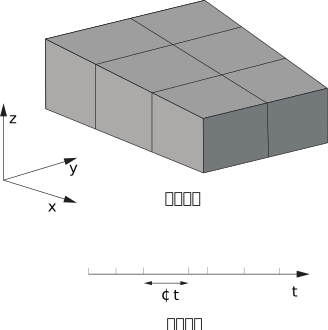
\includegraphics{fig-2-1}
 \caption{解析領域の離散化}
 \label{fig:2.1}
\end{figure}


\begin{figure}[ht]
 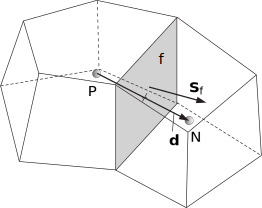
\includegraphics{fig-2-2}
 \caption{有限体積法の離散化におけるパラメータ}
 \label{fig:2.2}
\end{figure}


従属変数とその他の物理量は,たいていセル中心$P$で保存されますが,
面や点で保存される場合もあります.
セルは,一般に$f$とラベル付けされる平らな面で境界付けられます.
OpenFOAMでは,各セルをつくる面の数に制限はなく,
各面の配置にも制約はありません.
このような種類のメッシュは通常,
セルの面が所定の(例えば座標軸に沿った)配置になるメッシュと区別して,
「任意非構造」とよばれます.
任意非構造メッシュを採用したコードは,
領域の形状が複雑であったり時間変化する場合などは特に,
とても自由にメッシュの生成や操作を行うことができます.

ほとんどの物理量はセル中心で定義されますが,
セルの面で定義されるものもいくつかあります.
セルの面には二つのタイプがあります.
\begin{description}
 \item[内部面] 二つのセル(二つを上回ることはありません)をつなぐ面です.
            それぞれの内部面について,OpenFOAMは
            隣接するセルのうち一つをその面の「所有セル」,
            もう一方を「隣接セル」として指定します.
 \item[境界面] 一つだけのセルに属する面で,それゆえ領域の境界と一致します.
            これらの面には単純に所有セルしかありません.
\end{description}


\subsection{OpenFOAMにおけるメッシュ定義}
\label{ssec:2.3.1}
OpenFOAMにはいくつかの異なるレベルのメッシュ記述方法がありますが,
まずはもっとも基本的なメッシュクラスである\OFclass{polyMesh}について述べます.
多面体からなるので\OFclass{polyMesh}といいます.
\OFclass{polyMesh}は以下および\autoref{fig:2.2}に示すように,
メッシュ形状を定義するための最小限の情報で構成されます.
\begin{description}
 \item[点] 頂点の座標ベクトルのリスト,すなわち\OFclass{vectorField}ですが,
            改めて\texttt{typedef}宣言により\OFclass{pointField}と名付けられています.
 \item[面] セルの面のリスト\OFclass{List<face>},あるいは\OFclass{faceList}です.
            ここで,\OFclass{face}クラスは
            \OFclass{pointField}に対応する頂点番号のリストで定義されます.
 \item[セル] セルのリスト\OFclass{List<cell>}あるいは\OFclass{cellList}です.
            ここで,\OFclass{cell}クラスは
            上記の\OFclass{faceList}に対応する面番号のリストで定義されます.
 \item[境界] \OFclass{polyBoundaryMesh}は,境界の異なる領域を表すパッチのリスト
            \OFclass{polyPatchList}から成り立っています.
            このような方法で,解析の際に各々のパッチに
            異なる境界条件を適用できるように境界が細分化されます.
            あらゆる\OFclass{polyPatch}の全ての面は
            \OFclass{faceList}の一つのブロックに保存されており,
            ブロックの最初と最後の面への参照が保存された
            \OFclass{slice}クラスを使うことにより,
            それらの面に簡単にアクセスできます.
            それぞれの\OFclass{polyPatch}は以下から成り立っています.
            \begin{itemize}
             \item \OFclass{slice}
             \item 名前を付けるための\OFclass{word}
            \end{itemize}
\end{description}

有限体積法による離散化には,
\OFclass{polyMesh}に保存されている
メッシュ形状に由来する固有のデータが使われます.
そのためOpenFOAMでは,\OFclass{polyMesh}クラスを拡張した\OFclass{fvMesh}に,
有限体積法による離散化に必要な追加のデータが保存されます.
\OFclass{fvMesh}は{polyMesh}から構成され,
\autoref{tbl:2.1}に示すようなデータが保存されます.
これらのデータは,メッシュが動いたり細分化されたりする場合には,
実行時に更新することができます.


\begin{figure}[ht]
 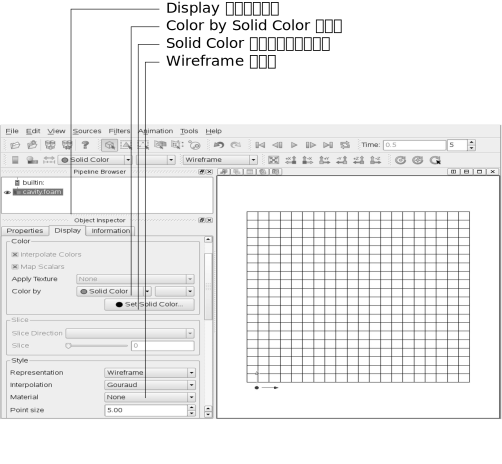
\includegraphics{fig-2-3}
 \caption{OpenFOAMにおける基本的なメッシュ表現の概略図}
 \label{fig:2.3}
\end{figure}


\begin{table}[ht]
 %#! uplatex ProgrammersGuideJa
\begin{tabular}{|c|c|c|c|}
 \hline
 \tblstrut
 クラス & 説明 & 記号 & アクセス関数 \\
 \hline\hline
 \tblstrut
 \OFclass{volScalarField} & セル体積 & $V$ & \verb|V()| \\
 \OFclass{surfaceVectorField} & 面の面積ベクトル & $\bm{S}_{\mathrm{f}}$ & \verb|Sf()| \\
 \OFclass{surfaceScalarField} & 面の面積の絶対値 & $|\bm{S}_{\mathrm{f}}|$ & \verb|magSf()| \\
 \OFclass{volVectorField} & セル中心 & $\bm{C}$ & \verb|C()| \\
 \OFclass{surfaceVectorField} & 面中心 & $\bm{C}_{\mathrm{f}}$ & \verb|Cf()| \\
 \OFclass{surfaceScalarField} & 面の運動流束 ** & $\phi_{\mathrm{g}}$ & \verb|phi()| \\
 \hline
\end{tabular}

 \caption{\OFclass{fvMesh}に保存されるデータ}
 \label{tbl:2.1}
\end{table}


\subsection{OpenFOAMにおける\OFclass{geometricField}の定義}
\label{ssec:2.3.2}
これまでのところ,場,すなわちテンソルのリスト,およびメッシュが定義できます.
これらを合わせることで,領域の離散点におけるテンソル場を定義することができます.
これはOpenFOAMにおいては,テンプレートクラス
\OFclass{geometricField<Type>}によって記述されます.
\OFclass{Field}の値は,
領域内部において例えばセル中心で定義されるものと,
領域の境界において例えば境界面上で定義されるものに分けられます.
\OFclass{geometricField<Type>}は以下のような情報を保存します.
\begin{description}
 \item[内部場] 単純に,\autoref{ssec:2.2.1}で述べたような
            \OFclass{Field<Type>}です.
 \item[境界場] これは\OFclass{GeometricBoundaryField}であり,その中では,
            それぞれのパッチの面について\OFclass{Field}が定義され,
            その境界のパッチについて\OFclass{Field}が定義されます.
            つまりこれは\OFclass{FieldField<Type>}クラスのオブジェクトに保存される,場の場です.
            また\OFclass{fvBoundaryMesh}への参照も保存されます.[**]
 \item[メッシュ] \OFclass{fvMesh}への参照ですが,
            その場がセル中心,面,などのうちどこで定義されているかに応じた
            いくつかの詳細情報も加わります.
 \item[次元] \href{../UserGuideJa/UserGuideJa.pdf#subsection.4.2.6}{ユーザガイドの4.2.6項}で述べる
            \OFclass{dimensionSet}です.
 \item[古い値] 時間微分の離散化には,前の時間ステップにおける場のデータが必要になります.
            \OFclass{geometricField<Type>}は,
            前の,一つ古い時間ステップ,および必要ならばその前の,二つ古い時間ステップ
            において保存された場のデータへの参照を保存しています.
 \item[前回の反復時の値] 反復解法の手順では不足緩和を利用できますが,
            これは前回の反復時のデータへのアクセスを必要とします.
            ここでも,必要であれば,\OFclass{geometricField<Type>}は
            前回の反復時のデータへの参照を保存します.
\end{description}
\autoref{sec:2.3}で述べたように,物理量はセル中心で定義することが主ですが,
セル面上で保存することもよくあり,セル頂点で定義することもときどきあります.
\OFclass{geometricField<Type>}は,場の変数がどこで定義されているかによって,
以下のように\texttt{typedef}宣言で改名されています.
\begin{description}
 \item[\OFclass{volField<Type>}] 場がセル中心で定義されているとき
 \item[\OFclass{surfaceField<Type>}] 場がセルの面で定義されているとき
 \item[\OFclass{pointField<Type>}] 場がセルの頂点で定義されているとき
\end{description}

これらの\OFclass{geometricField<Type>}から
\texttt{typedef}された場のクラスは\autoref{fig:2.4}に図示されています.
\OFclass{geometricField<Type>}は\OFclass{Field<Type>}のテンソル代数を全て継承しており,
全ての演算は\OFclass{dimensionSet}の次元チェックに従います.
また次節で述べる有限体積法の離散化手順にも依存することがあります.
\OFclass{geometricField<Type>}を作るときに使われるクラス構造は\autoref{fig:2.5}%
\footnote{この図はクラス階層を厳密に表したものではなく,
むしろいくつかの原始クラスを\OFclass{geometricField<Type>}につながる
一般的な構造を表したものです.}%
に図示されています.


\begin{figure}[ht]
 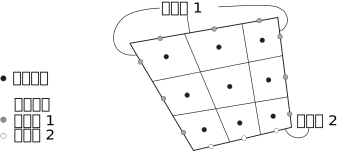
\includegraphics{fig-2-4-a}\par
 \medskip
 (a) \OFclass{volField<Type>}\par
 \bigskip
 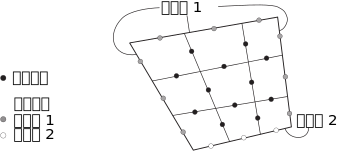
\includegraphics{fig-2-4-b}\par
 \medskip
 (b) \OFclass{surfaceField<Type>}\par
 \bigskip
 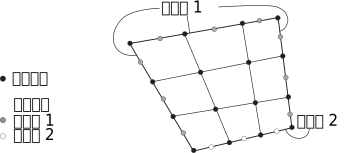
\includegraphics{fig-2-4-c}\par
 \medskip
 (c) \OFclass{pointField<Type>}\par
 \medskip
 \caption{二つの境界パッチをもつメッシュ上で定義された
 \OFclass{geometricField<Type>}のタイプ(簡単のため2次元で表している)}
 \label{fig:2.4}
\end{figure}


\begin{figure}[ht]
 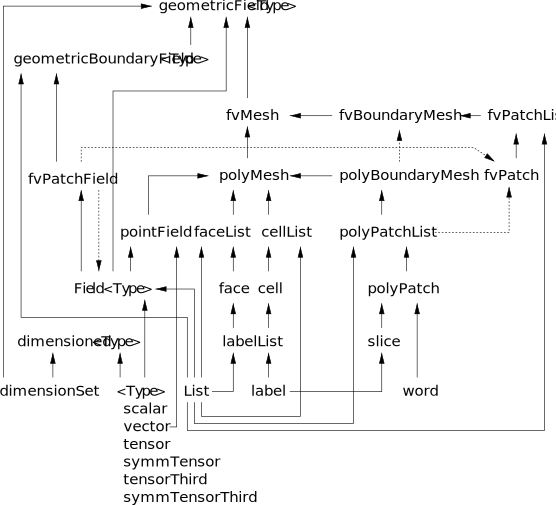
\includegraphics{fig-2-5}
 \caption{\OFclass{geometricField<Type>}につながる基本的なクラス構造}
 \label{fig:2.5}
\end{figure}


\section{方程式の離散化}
\label{sec:2.4}
方程式の離散化により,偏微分方程式は一般に以下のような行列で表される代数方程式に変換されます.
\begin{align}
 \label{eq:2.12}
 [A][x] = [b]
\end{align}
ここで$[A]$は正方行列,$[x]$は従属変数の列ベクトル,$[b]$はソースベクトルです.
$[x]$と$[b]$は,その形状,例えば\OFclass{geometricField<Type>},
またはもっと厳密には,有限体積法による離散化を用いているならば\OFclass{volField<Type>}の
各位置で定義された値のリストという本来の正確な表現ではなく,
むしろ行列用語でいう「ベクトル」です.

$[A]$は代数式群の係数のリストであり,\OFclass{geometricField<Type>}では記述できません.
したがって,独自のクラス\OFclass{fvMatrix}で与えられます.
\OFclass{fvMatrix<Type>}は\OFclass{geometric<Type>Field}の離散化によって生成され,
したがって\OFclass{<Type>}を継承します.
これは,加算\hskip\xkanjiskip\verb|+|,
減算\hskip\xkanjiskip\verb|-|\hskip\xkanjiskip
そして乗算\hskip\xkanjiskip\verb|*|\hskip\xkanjiskip
という標準的な行列の代数演算の多くをサポートします.

OpenFOAMのコードにおいて偏微分方程式の各項は,
それぞれ静的な関数のクラス\OFclass{finiteVolumeMethod}や
\OFclass{finiteVolumeCalculus}を用いて記述されます.
これらのクラスは\texttt{typedef}によって,それぞれ\OFclass{fvm}および\OFclass{fvc}と略されます.
\OFclass{fvm}や\OFclass{fvc}は,
例えば$\nabla^{2}$,$\nabla \inProd {}$および$\partial/\partial t$といった
\OFclass{geometricField<Type>}を離散化する微分演算子を表す静的な関数を備えています.
これらの関数を,一つではなく二つのクラス\OFclass{fvm}と\OFclass{fvc}で定義しているのは,
以下のように区別するためです.
\begin{itemize}
 \item \OFclass{fvm}の関数は陰的な微分を計算し,\OFclass{fvMatrix<Type>}を返す.
 \item \OFclass{fvc}のいくつかの関数は陽的な微分を計算,その他は陽的な計算をし,
       \OFclass{geometricField<Type>}を返す.
\end{itemize}
\autoref{fig:2.6}には,
二つの境界パッチをもつメッシュ上で定義された\OFclass{geometricField<Type>}を示しており,
陽的な演算が単にある場を他の場に変換するだけであることを表しています.
簡単のために2次元で描いています.


\begin{figure}[ht]
 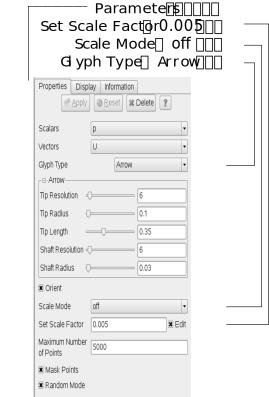
\includegraphics{fig-2-6}
 \caption{\OFclass{geometricField<Type>}とその演算}
 \label{fig:2.6}
\end{figure}


\OFclass{fvm}および\OFclass{fvc}で使える,偏微分方程式の項を離散化する主な関数を
\autoref{tbl:2.2}にリストアップしています.
各項の有限体積法による離散化は,ガウスの定理により,
その体積を囲んでいるセル表面の面積分に変換されます.
\begin{align}
 \label{eq:2.13}
 \int_{V}\nabla \star \phi\,\mathrm{d}V
 = \int_{S}\mathrm{d}\bm{S} \star \phi
\end{align}
ここで$\bm{S}$は表面積ベクトル,$\phi$は任意のテンソル場,
そして$\star$はテンソル任意の乗算,例えば内積,外積,クロス積,
およびそれぞれの微分,発散$\nabla \inProd \phi$,
勾配$\nabla\phi$および$\nabla \times \phi$を表しています.
次に,体積および面積分は各項について後述するような適切なスキームで線形化されます.
OpenFOAMでは,いくつかの項は常に同じスキームで離散化されますが,
その他の項の離散化についてはスキームの選択肢が提供されています.
スキームの選択はコードの中で直接指定することもできますし,
ジョブの実行時にインプットファイルから読み込んで
\OFclass{fvSchemes}クラスのオブジェクトとして保持する方法もあります.


\begin{table}[ht]
 %#! platex ProgrammersGuideJa
\begin{tabular}{|cccc|}
 \hline
 項の記述 & 陰的・陽的 & 記述 & \OFclass{fvm::}または\OFclass{fvc::}の関数 \\
 \hline\hline
 ラプラシアン & 陰的・陽的 & $\nabla^{2}\phi$ & \texttt{laplacian(phi)} \\
 &  & $\nabla \inProd \varGamma \nabla \phi$ & \texttt{laplacian(Gamma, phi)} \\
 \hline
 時間微分 & 陰的・陽的 & $\frac{\partial\phi}{\partial t}$ & \texttt{ddt(phi)} \\
 &  & $\frac{\partial\rho\phi}{\partial t}$ & \texttt{ddt(rho, phi)} \\
 \hline
 時間の2階微分 & 陰的・陽的 & $\frac{\partial}{\partial t}\left(\rho\frac{\partial\phi}{\partial t}\right)$ & \texttt{d2dt2(rho, phi)} \\
 \hline
 移流 & 陰的・陽的 & $\nabla \inProd (\psi)$ & \verb|div(psi, scheme)*| \\
 &  & $\nabla \inProd (\psi\phi)$ & \verb|div(psi, phi, word)*| \\
 &  &  & \verb|div(psi, phi)| \\
 \hline
 発散 & 陽的 & $\nabla \inProd \chi$ & \texttt{div(chi)} \\
 \hline
 勾配 & 陽的 & $\nabla \chi$ & \texttt{grad(chi)} \\
 &  & $\nabla \phi$ & \texttt{gGrad(phi)} \\
 &  &  & \texttt{lsGrad(phi)} \\
 &  &  & \texttt{snGrad(phi)} \\
 &  &  & \texttt{snGradCorrection(phi)} \\
 \hline
 勾配の勾配の二乗 & 陽的 & $|\nabla\nabla\phi|^{2}$ & \texttt{sqrGradGrad(phi)} \\
 \hline
 回転 & 陽的 & $\nabla \times \phi$ & \texttt{curl(phi)} \\
 \hline
 湧き出し & 陰的 & $\rho\phi$ & \texttt{Sp(rho, phi)} \\
 & 陰的・陽的\textsuperscript{\dag} &  & \texttt{SuSp(rho, phi)} \\
 \hline
 \multicolumn{4}{l}{\dag\ 湧き出し\OFkeyword{fvm::SuSp}は
 \OFkeyword{rho}の符号に依存して,陰的または陽的に離散化されます.} \\
 \multicolumn{4}{l}{\dag\ 陽的な湧き出しは単純に
 \OFclass{vol<Type>Field}で指定されます.例:\texttt{rho*phi}} \\
 \multicolumn{4}{l}{関数の引数は以下のようなクラスです.} \\
 \multicolumn{4}{l}{\OFkeyword{phi}: \OFclass{vol<Type>Field}} \\
 \multicolumn{4}{l}{\OFkeyword{Gamma}: \OFclass{scalar},\OFclass{volScalarField},
 \OFclass{volTensorField},\OFclass{surfaceTensorField}.} \\
 \multicolumn{4}{l}{\OFkeyword{rho}: \OFclass{scalar},\OFclass{volScalarField}} \\
 \multicolumn{4}{l}{\OFkeyword{psi}: \OFclass{surfaceTensorField}} \\
 \multicolumn{4}{l}{\OFkeyword{chi}: \OFclass{surface<Type>Field},\OFclass{vol<Type>Field}} \\
\end{tabular}

 \caption{OpenFOAMにおける偏微分方程式の項の離散化}
 \label{tbl:2.2}
\end{table}


\subsection{ラプラシアン項}
\label{ssec:2.4.1}
ラプラシアンの項は,以下のように検査体積で積分・線形化されます.
\begin{align}
 \label{eq:2.14}
 \int_{V}\nabla \inProd (\varGamma\nabla\phi)\,\mathrm{d}V
 = \int_{S}\mathrm{d}\bm{S} \inProd (\varGamma\nabla\phi)
 = \sum_{f}\varGamma_{f}\bm{S}_{f} \inProd (\nabla\phi)_{f}
\end{align}
みているセル$P$の中心と隣のセル$N$の中心の間の長さベクトル$\bm{d}$が
そのフェイス面に垂直,すなわち$\bm{S}_{f}$に平行ならば,
面の勾配の離散化は陰的になります.
\begin{align}
 \label{eq:2.15}
 \bm{S}_{f} \inProd (\nabla\phi)_{f}
 = |S_{f}|\frac{\phi_{N} - \phi_{P}}{|\bm{d}|}
\end{align}
非直交メッシュの場合,
セル中心勾配(これはセル中心値の中心差分から計算される)の
内挿によって評価される陽的な項が加わります.


\subsection{対流項}
\label{ssec:2.4.2}
対流項は,以下のように検査体積で積分・線形化されます.
\begin{align}
 \label{eq:2.16}
 \int_{V}\nabla \inProd (\rho\bm{U}\phi)\,\mathrm{d}V
 = \int_{S}\mathrm{d}\bm{S} \inProd (\rho\bm{U}\phi)
 = \sum_{f}\bm{S}_{f} \inProd (\rho\bm{U})_{f}\phi_{f}
 = \sum_{f}F\phi_{f}
\end{align}

表面の場$\phi_{f}$はさまざまなスキームで評価されます.
\begin{description}
 \item[中心差分 (CD)] は,2次精度ですが不安定です.
            \begin{align}
             \label{eq:2.17}
             \phi_{f} = f{x}\phi_{P} + (1 - f_{x})\phi_{N}
            \end{align}
            ここで$f_{x} \equiv \overline{fN}/\overline{PN}$,
            $\overline{fN}$は$f$とセル中心$N$の距離,
            $\overline{PN}$はセル中心同士$P$と$N$の距離です.
 \item[風上差分 (UD)] は,流れの方向から$\phi_{f}$を決定し,
            精度は犠牲になりますが安定です.
            \begin{align}
             \label{eq:2.18}
             \phi_{f} =
             \begin{cases}
              \phi_{P} & F \ge 0 \text{のとき} \\
              \phi_{N} & F < 0 \text{のとき}
             \end{cases}
            \end{align}
 \item[ブレンド差分 (BD)] スキームは,適切な精度で
            安定性を保つことを狙ってUDとCDを組み合わせます.
            \begin{align}
             \phi_{f} = (1 - \gamma)(\phi_{f})_{\mathrm{UD}} + \gamma(\phi_{f})_{\mathrm{CD}}
            \end{align}
            OpenFOAMには,ブレンド係数$\gamma$を選ぶGamma差分スキームのいくつかの実装がありますが,
            それはほかのよく知られたスキーム,van Leer,SUPERBEE,MINMODなどを表しています.
\end{description}


\subsection{1階の時間微分}
\label{ssec:2.4.3}
1階の時間微分$\partial/\partial t$は,以下のように検査体積で積分されます.
\begin{align}
 \label{eq:2.20}
 \frac{\partial}{\partial t}\int_{V}\rho\phi\,\mathrm{d}V
\end{align}
この項は,以下のものを使って時間に関して単純な差分で離散化されます.
\begin{description}
 \item[新しい値] いま解いている時間ステップの値$\phi^{n} \equiv \phi(t + \Delta t)$
 \item[古い値] 前の時間ステップで保存された値$\phi^{o} \equiv \phi(t)$
 \item[二つ古い値] 二つ前の時間ステップで保存された値$\phi^{oo} \equiv \phi(t - \Delta t)$
\end{description}
\href{../UserGuideJa/UserGuideJa.pdf#section.4.4}{ユーザガイドの4.4節}に詳しく述べられているように,
該当する入力ファイルの中で\OFkeyword{timeScheme}キーワードを使って,
二つのうち一つの離散化スキームを宣言することができます.
\begin{description}
 \item[オイラーの陰解法] スキーム,\OFkeyword{timeScheme EulerImplicit},
            これは時間に関して1次精度です.
            \begin{align}
             \label{eq:2.21}
             \frac{\partial}{\partial t}\int_{V}\rho\phi\,\mathrm{d}V
             = \frac{(\rho_{P}\phi_{P}V)^{n} - (\rho_{P}\phi_{P}V)^{o}}{\Delta t}
            \end{align}
 \item[後退差分] スキーム,\OFkeyword{timeScheme BackwardDifferencing},
            これは二つ前の値を保存することにより時間に関して2次精度であり,
            したがって\OFkeyword{EulerImplicit}よりデータ保存のオーバーヘッドが大きくなります.
            \begin{align}
             \label{eq:2.22}
             \frac{\partial}{\partial t}\int_{V}\rho\phi\,\mathrm{d}V
             = \frac{3(\rho_{P}\phi_{P}V)^{n} - 4(\rho_{P}\phi_{P}V)^{o}
             + (\rho_{P}\phi_{P}V)^{oo}}{2\Delta t}
            \end{align}
\end{description}


\subsection{2階の時間微分}
\label{ssec:2.4.4}
2階の時間微分は,以下のように検査体積で積分・線形化されます.
\begin{align}
 \label{eq:2.23}
 \frac{\partial}{\partial t}\int_{V}\rho\frac{\partial\phi}{\partial t}\,\mathrm{d}V
 = \frac{(\rho_{P}\phi_{P}V)^{n} - 2(\rho_{P}\phi_{P}V)^{o}
 + (\rho_{P}\phi_{P}V)^{oo}}{\Delta t^{2}}
\end{align}
これは時間について1次精度です.


\subsection{発散}
\label{ssec:2.4.5}
この節で述べる発散項は,
\autoref{ssec:2.4.2}の対流項とは区別される完全に陽的な項です.
つまり対流項は,速度とある従属変数の積の発散ではありません.
この項は以下のように検査体積で積分・線形化されます.
\begin{align}
 \label{eq:2.24}
 \int_{V}\nabla \inProd \phi\,\mathrm{d}V
 = \int_{S}\mathrm{d}\bm{S} \inProd \phi
 = \sum_{f}\bm{S}_{f} \inProd \phi_{f}
\end{align}
\OFkeyword{fvc::div}関数は\OFclass{surface<Type>}または
\OFclass{vol<Type>Field}のどちらも引数にとることができます.
前者では$\phi_{f}$は直接与えられ,
後者では\autoref{ssec:2.4.10}で述べる中心差分で値が面上に内挿されます.


\subsection{勾配}
\label{ssec:2.4.6}
勾配の項は様々な方法で評価できる陽的な項です.
そのスキームは,例えば\OFkeyword{fvc::gGrad},\OFkeyword{fvc::lsGrad}などのような
離散化スキームに対して適切な特定の勾配関数を選ぶか,
または入力ファイルの中の適切な\OFkeyword{timeScheme}キーワードに
連動した\OFkeyword{fvc::grad}関数を使うか,
いずれの方法でも評価できます.
\begin{description}
 \item[ガウス積分] は,\OFkeyword{fvc::grad}関数を
            \OFkeyword{timeScheme Gauss}と合わせて使うことで動作します.
            この離散化は体積分に対してガウスの定理を適用する標準的な手法を使います.
            \begin{align}
             \label{eq:2.25}
             \int_{V}\nabla\phi\,\mathrm{d}V
             = \int_{S}\mathrm{d}\bm{S}\phi
             = \sum_{f}\bm{S}_{f}\phi_{f}
            \end{align}
 \item[最小二乗法] は,以下の考えに基づいています.
            \begin{enumerate}
             \item 点$P$における値を,点$P$における勾配を使って隣の点$N$に外挿する.
             \item 点$N$に外挿された値を,点$N$における実際の値と比較,この差が誤差となる.
             \item 点$P$の付近の全ての点における誤差を,
                   それぞれの勾配で重み付けして二乗した総和を最小化すれば,
                   勾配の良い近似値が得られる.
            \end{enumerate}
            最小二乗法は\OFkeyword{fvc::grad}関数を
            \OFkeyword{timeScheme leastSquares}と組み合わせるか,
            直接\OFkeyword{fvc::lsGrad}を使うことで動作します.
            この離散化は,まず全ての点$P$において,その近隣の点$N$での総和を求めて,
            テンソル$\bm{G}$を計算します.
            \begin{align}
             \label{eq:2.26}
             \bm{G} = \sum_{N}w_{N}^{2}\bm{d}\bm{d}
            \end{align}
            ここで$\bm{d}$は$P$から$N$へのベクトルであり,
            重み関数は$w_{N} = 1/|\bm{d}|$です.
            勾配は以下のように評価されます.
            \begin{align}
             \label{eq:2.27}
             (\nabla\phi)_{P}
             = \sum_{N}w_{N}^{2}\bm{G}^{-1} \inProd \bm{d}(\phi_{N} - \phi_{P})
            \end{align}
 \item[面に垂直な勾配] 面に垂直な勾配$\bm{n}_{f} \inProd (\nabla\phi)_{f}$は
            セルの面において以下のスキームを使って評価できます.
            \begin{align}
             \label{eq:2.28}
             (\nabla\phi)_{f} = \frac{\phi_{N} - \phi_{P}}{|\bm{d}|}
            \end{align}
            この勾配は\OFkeyword{fvc::snGrad}関数で呼び出され,
            \OFclass{surfaceField<Type>}を返します.
            このスキームは\autoref{ssec:2.4.1}で述べた
            ラプラシアンの離散化スキームと似た方法で直接評価され,
            また同じように非直交メッシュの場合には,
            この面の勾配の精度を高めるために補正が加えられます.
            この補正は\OFkeyword{fvc::snGradCorrection}関数を使って呼び出されます.
            [Check**]
\end{description}


\subsection{勾配の勾配の平方}
\label{ssec:2.4.7}
勾配の勾配の平方の項は,場の勾配をとり,得られた勾配場の勾配をとり,
そしてその結果の絶対値二乗を計算することで評価されます.
$\phi$の勾配の勾配の平方を数式で書くと$|\nabla (\nabla\phi)|^{2}$となります.


\subsection{回転}
\label{ssec:2.4.8}
回転は,\autoref{ssec:2.4.6}で述べた勾配の項から評価されます.
まず勾配が離散化され,それから\autoref{eq:2.7}の関係(以下に再掲)を
使って回転が評価されます.
\begin{align*}
 \nabla \times \phi = 2 \mathop{*} (\mathop{\mathrm{skew}}\nabla\phi)
\end{align*}


\subsection{湧き出し項}
\label{ssec:2.4.9}
湧き出し項は三つの方法で指定できます.
\begin{description}
 \item[陽解法] すべての陽的な項は\OFclass{volField<Type>}です.
            したがって,陽的な湧き出し項は単純に値の場として等式の中に組み込まれます.
            例えば,\OFkeyword{phi}と\OFkeyword{f}を\OFclass{volScalarField}として定義し,
            そして以下のようにします.
            \begin{OFverbatim}[file]
solve(fvm::laplacian(phi) == f)
            \end{OFverbatim}
 \item[陰解法] 陰的な湧き出し項は,以下のように検査体積で積分・線形化されます.
            \begin{align}
             \label{eq:2.29}
             \int_{V}\rho\phi\,\mathrm{d}V = \rho_{P}V_{P}\phi_{P}
            \end{align}
 \item[陰・陽解法] 陰的な湧き出し項は,行列の対角成分の係数を変えます.
            その係数と行列の項の符号に依存して,
            これは行列の対角成分の支配力を増大または減少させます.
            対角成分の支配力を減少させることは,
            行列の方程式の反復解法の際の不安定さを引き起こします.
            したがって,OpenFOAMは混成の湧き出し項の離散化方法を提供しており,
            これは係数が正のとき陰的に,負のときには陽的になります.
            数式上は,点$P$に対する行列の係数は$V_{P}\max(\rho_{P},\ 0)$,
            そして湧き出し項は$V_{P}\phi_{P}\min(\rho_{P},\ 0)$となります.
\end{description}


\subsection{その他の陽的な離散化スキーム}
\label{ssec:2.4.10}

他にも\OFclass{volField<Type>}を\OFclass{surface<Type>Field}に,
および逆に変換する離散化手法がいくつかあります.
\begin{description}
 \item[面積分] \OFkeyword{fvc::surfaceIntegrate}は,
            それぞれのセルを区切る面での値\OFclass{surface<Type>Field}の総和をとり,
            セルの体積で割るという操作をします.
            すなわち$(\sum_{f}\phi_{f})/V_{P}$となります.
            これは\OFclass{volField<Type>}を返します.
 \item[面総和] \OFkeyword{fvc::surfaceSum}は,
            それぞれのセルを区切る面での値\OFclass{surface<Type>Field}の総和をとる操作です.
            すなわち$\sum_{f}\phi_{f}$となり,
            \OFclass{volField<Type>}を返します.
 \item[平均値] \OFkeyword{fvc::average}は,
            面の値\OFclass{surface<Type>Field}の面積重み付け平均をとります.
            すなわち$(\sum_{f}S_{f}\phi_{f})/\sum_{f}S_{f}$となり,
            \OFclass{volField<Type>}を返します.
 % \item[Reconstruct] 
 \item[面内挿] \OFclass{geometric<Type>Field}の関数\OFkeyword{faceInterpolate()}は,
            セル中心の値\OFclass{volField<Type>}を,
            中心差分を使ってセルの面上へ内挿し,\OFclass{surface<Type>Field}を返します.
\end{description}



\section{時間微分}
\label{sec:2.5}
時間微分の離散化については\autoref{ssec:2.4.3}および\autoref{ssec:2.4.4}で述べましたが,
非定常問題における空間微分の扱い方について考える必要があります.
もし$\mathcal{A}$を任意の空間微分演算子,
例えばラプラシアン,として,
あらゆる空間微分を$\mathcal{A}\phi$で表すとすれば,
非定常の偏微分方程式を積分型で以下のように表記できます.
\begin{align}
 \label{eq:2.30}
 \int_{t}^{t + \Delta t}\left[\frac{\partial}{\partial t}\int_{V}\rho\phi\,\mathrm{d}V
 + \int_{V}\mathcal{A}\phi\,\mathrm{d}V\right]\mathrm{d}t = 0
\end{align}
\autoref{eq:2.21}のオイラー陰解法を使うと,第1項は次のように書けます.
\begin{align}
 \label{eq:2.31}
 \int_{t}^{t + \Delta t}
 \left[\frac{\partial}{\partial t}\int_{V}\rho\phi\,\mathrm{d}V\right]\mathrm{d}t
 &= \int_{t}^{t + \Delta t}
 \frac{(\rho_{P}\phi_{P}V)^{n} - (\rho_{P}\phi_{P}V)^{o}}{\Delta t}\mathrm{d}t \\
 &= \frac{(\rho_{P}\phi_{P}V)^{n} - (\rho_{P}\phi_{P}V)^{o}}{\Delta t}\Delta t
\end{align}

第2項は次のように書けます.
\begin{align}
 \label{eq:2.32}
 \int_{t}^{t + \Delta t}\left[\int_{V}\mathcal{A}\phi\,\mathrm{d}V\right]\mathrm{d}t
 = \int_{t}^{t + \Delta t}\mathcal{A}^{*}\phi\,\mathrm{d}t
\end{align}
ここで$\mathcal{A}^{*}$は空間で離散化した$\mathcal{A}$を表します.
時間積分は三つの方法で離散化できます.
\begin{description}
 \item[オイラー陰解法] 空間については陰解法で離散化し,したがって現在の値$\phi^{n}$をとります.
            \begin{align}
             \label{eq:2.33}
             \int_{t}^{t + \Delta t}\mathcal{A}^{*}\phi\,\mathrm{d}t
             = \mathcal{A}^{*}\phi^{n}\Delta t
            \end{align}
            これは時間について1次精度であり,有界性と無条件安定性を保証します.
 \item[陽解法] 空間については陽解法で離散化し,したがって前の時刻の値$\phi^{o}$をとります.
            \begin{align}
             \label{eq:2.34}
             \int_{t}^{t + \Delta t}\mathcal{A}^{*}\phi\,\mathrm{d}t
             = \mathcal{A}^{*}\phi^{o}\Delta t
            \end{align}
            これは時間について1次精度であり,もしクーラン数$\nCo$が$1$より大きければ不安定です.
            クーラン数は以下のように定義されます.
            \begin{align}
             \label{eq:2.35}
             \nCo = \frac{\bm{U}_{f} \inProd \bm{d}}{|\bm{d}|^{2}\Delta t}
            \end{align}
            ここで$\bm{U}_{f}$は代表速度,例えば波面の速度,流れの速度などです.
 \item[クランク・ニコルソン法] 空間の項の離散化に台形公式を使い,
            したがって現在の値$\phi^{n}$と前の時刻の値$\phi^{o}$の平均値をとります.
            \begin{align}
             \label{eq:2.36}
             \int_{t}^{t + \Delta t}\mathcal{A}^{*}\phi\,\mathrm{d}t
             = \mathcal{A}^{*}\left(\frac{\phi^{n} + \phi^{o}}{2}\right)\Delta t
            \end{align}
            これは時間について2次精度であり,無条件で安定ですが,有界性は保証されません.
\end{description}


\subsection{OpenFOAMにおける時間微分の取扱い}
\label{ssec:2.5.1}
現在のところ,時間の離散化の取り扱いは,
解くべき偏微分方程式における空間微分の実装によって制御されます.
例えば,非定常の拡散方程式を解きたいとします.
\begin{align}
 \label{eq:2.37}
 \frac{\partial\phi}{\partial t} = \kappa\nabla^{2}\phi
\end{align}
これに対するオイラーの陰解法は以下のようになります.
\begin{OFverbatim}[file]
solve(fvm::ddt(phi) == kappa*fvm::laplacian(phi))
\end{OFverbatim}
ここで\OFkeyword{Laplacian}の項を陰解法で離散化するために\OFclass{fvm}クラスを使います.
陽解法で実装するには以下のようにします.
\begin{OFverbatim}[file]
solve(fvm::ddt(phi) == kappa*fvc::laplacian(phi))
\end{OFverbatim}
今度は\OFkeyword{Laplacian}の項を陽解法で離散化するために\OFclass{fvc}クラスを使います.
クランク・ニコルソン・スキームは,陰解法と陽解法の平均をとることで実装できます.
\begin{OFverbatim}[file]
solve
    (
    fvm::ddt(phi)
    ==
    kappa*0.5*(fvm::laplacian(phi) + fvc::laplacian(phi))
    )
\end{OFverbatim}



\section{境界条件}
\label{sec:2.6}
解きたい問題を完成させるためには境界条件が必要です.
したがって全ての境界面において境界条件を指定しなければなりません.
境界条件は二つのタイプに分けられます.
\begin{description}
 \item[ディリクレ条件] は,その従属変数の境界における値を定めます.
            したがって,このガイドでは「固定値」とよびます.
            % したがって,このガイドでは `fixed value' とよびます.
 \item[ノイマン条件] は,その従属変数の境界に垂直な勾配を定めます.
            したがって,このガイドでは「固定勾配」とよびます.
            % したがって,このガイドでは `fixed gradient' とよびます.
\end{description}

面にわたる総和$\sum_{f}$を含む項の離散化を行うときには,
それらの面のうちの一つが境界面であったらどうなるかを考慮する必要があります.
\begin{description}
 \item[固定値] 境界における値$\phi_{b}$を指定
            \begin{itemize}
             \item 離散化に,境界面における値$\phi_{f}$を使う場合は,
                   単純に$\phi_{b}$で置き換えることができます.
                   例えば\autoref{eq:2.16}の移流項の場合です.
             \item 面における勾配$(\nabla\phi)_{f}$が必要な項,
                   例えばラプラシアンなど,の場合には,
                   その勾配は境界面における値とセル中心の値を使って計算されます.
                   \begin{align}
                    \label{eq:2.38}
                    \bm{S}_{f} \inProd (\nabla\phi)_{f}
                    = |S_{f}|\frac{\phi_{b} - \phi_{P}}{|\bm{d}|}
                   \end{align}
            \end{itemize}
 \item[固定勾配] 固定勾配境界条件$g_{b}$は,
            勾配と,境界の単位法線ベクトルとの内積になります.
            \begin{align}
             \label{eq:2.39}
             g_{b} = \left(\frac{\bm{S}}{|\bm{S}|} \inProd \nabla\phi\right)_{f}
            \end{align}
            \begin{itemize}
             \item 離散化に,境界面における値$\phi_{f}$を使う場合は,
                   セル中心の値を境界上に内挿する必要があります.
                   \begin{align}
                    \label{eq:2.40}
                    \phi_{f}
                    &= \phi_{P} + \bm{d} \inProd (\nabla\phi)_{f} \notag \\
                    &= \phi_{P} + |\bm{d}|g_{b}
                   \end{align}
             \item 離散化に面の勾配が評価される場合は,
                   直接$g_{b}$で置き換えることができます.
                   \begin{align}
                    \label{eq:2.41}
                    \bm{S}_{f} \inProd (\nabla\phi)_{f} = |S_{f}|g_{b}
                   \end{align}
            \end{itemize}
\end{description}


\subsection{物理的な境界条件}
\label{ssec:2.6.1}
境界条件の指定は通常,本当の振る舞いに対するエンジニアの解釈です.
現実の境界条件は一般に,
前節で述べたような数値的記述ではなく,
物理的な特性によって定義されます.
非圧縮性流体の流れでは,以下のような物理的な境界があります.
\begin{description}
 \item[入口] 入口における速度場が与えられ,それと整合させるために,
            圧力の境界条件は勾配ゼロになります.
 \item[出口] 出口における圧力場が与えられ,
            速度には勾配ゼロ境界条件が指定されます.
 \item[滑りなし不浸透性壁面] 流体の速度は壁面自身の速度と等しくなり,
            したがって,固定値条件が指定されます.
            壁を通り抜ける流束がゼロであることから,
            圧力は勾配ゼロが指定されます.
\end{description}

解の領域と境界条件がある面について対称となるような問題では,
その対称面の片側の半分の領域だけしかモデル化する必要はありません.
その面の境界条件は以下に従って指定しなければなりません.
\begin{description}
 \item[対称面] 対称面条件は,その面に垂直な勾配成分をゼロと指定します.[Check**]
\end{description}

../../../ProgrammersGuideJa/chapter3.tex

\backmatter
\makeatletter
\def\@linkcolor{blue}%
\makeatother
\printindex

\end{document}
